\chapter*{Appendix: Preview of group activity}
		\addcontentsline{toc}{chapter}{Appendix: Preview of group activity}
		
		\section*{Meeting log}
		
		\textbf{\textit{Kontinuirano osvježavanje}}\\

		
		\begin{packed_enum}
			\item  Meeting
			

			\item[] \begin{packed_item}
				\item Date: October 4, 2019
				\item Attended: P.Fribert, D.R.Sparemblek, B.Bilic, K.Ceple, D.Strbad, L.Lendel, K.Jezic
				\item Meeting theme:
				\begin{packed_item}
					\item  initial getting to know each other, individual skills
				\end{packed_item}
			\end{packed_item}
			\item  Meeting
			\item[] \begin{packed_item}
				\item Date: October 5, 2019
				\item Attended: P.Fribert, D.R.Sparemblek, B.Bilic, K.Ceple, D.Strbad, L.Lendel, K.Jezic
				\item Meeting theme:
				\begin{packed_item}
					\item  creating back end, front end and server team
				\end{packed_item}
			\end{packed_item}
			\item  Meeting
			\item[] \begin{packed_item}
				\item Date: October 15, 2019
				\item Attended:D.R.Sparemblek, B.Bilic
				\item Meeting theme:
				\begin{packed_item}
					\item  making first draft database
				\end{packed_item}
			\end{packed_item}
			\item  Meeting
			\item[] \begin{packed_item}
				\item Date: October 23, 2019
				\item Attended:D.R.Sparemblek, B.Bilic, P.Fribert
				\item Meeting theme:
				\begin{packed_item}
					\item  making database in python
				\end{packed_item}
			\end{packed_item}
			\item  Meeting
			\item[] \begin{packed_item}
				\item Date: October 24, 2019
				\item Attended:L.Lendel, B.Bilic, K.Jezic, D.R.Šparemblek, P.Fribert
				\item Meeting theme:
				\begin{packed_item}
					\item  signup and login screen functions
				\end{packed_item}
			\end{packed_item}
			\item  Meeting
			\item[] \begin{packed_item}
				\item Date: November 6, 2019
				\item Attended: P.Fribert, D.R.Sparemblek
				\item Meeting theme:
				\begin{packed_item}
					\item  foreign keys in database
				\end{packed_item}
			\end{packed_item}
			\item  Meeting
			\item[] \begin{packed_item}
				\item Date: November 7, 2019
				\item Attended: P.Fribert, B.Bilic, K.Ceple, D.Strbad, L.Lendel, K.Jezic
				\item Meeting theme:
				\begin{packed_item}
					\item  server functions
					\item  front end: hashing passwords and checking emails
					\item  documentation update
				\end{packed_item}
			\end{packed_item}
			\item  Meeting
			\item[] \begin{packed_item}
				\item Date: November 10, 2019
				\item Attended: D.R.Sparemblek, B.Bilic, L.Lendel, K.Jezic
				\item Meeting theme:
				\begin{packed_item}
					\item  debugging application, checking code
				\end{packed_item}
			\end{packed_item}
			\item  Meeting
			\item[] \begin{packed_item}
				\item Date: November 11, 2019
				\item Attended: P.Fribert, D.R.Sparemblek, B.Bilic, K.Ceple, D.Strbad, L.Lendel, K.Jezic
				\item Meeting theme:
				\begin{packed_item}
					\item  final changes before commiting project
				\end{packed_item}
			\end{packed_item}
			
			\item  Meeting
			\item[] \begin{packed_item}
				\item Date: November 13, 2019
				\item Attended: P.Fribert, K.Ceple
				\item Meeting theme:
				\begin{packed_item}
					\item  documentation specifics
				\end{packed_item}
			\end{packed_item}
			
			\item On further meetings: There were a lot further meetings, whose details we did not note down, and have forgotten about. We(especially some group members) had very frequent meetings with intertwining and diverse themes, so it is hard to pinpoint and remember what and when was exactly done. It is possible to give an outline though:
			
			\item Pre-winter break
			\item Implemented:
			\item[] \begin{packed_enum}
				\item OAuth 2.0
				\item XML Designs
				\item Project redesign - MVC applied
				\item Skeleton project set-up
				\item Log-in and register fixed
				\item Basic functionalities implemented
			\end{packed_enum}
			
			\item Start of January - Implemented most of the functionalities
			
			\item The first week of post-winter break: debugging and more additions
			\item Second week: further debugging, completing, documentation
			%
			
		\end{packed_enum}
		
		\eject
		\section*{Activity table}
		
			\textbf{\textit{Continuously refreshed}}\\
	
			\begin{longtabu} to \textwidth {|X[7, l]|X[1, c]|X[1, c]|X[1, c]|X[1, c]|X[1, c]|X[1, c]|X[1, c]|}
								
				\cline{2-8} \multicolumn{1}{c|}{\textbf{}} &     \multicolumn{1}{c|}{\rotatebox{90}{\textbf{Bartol Bilic}}} & \multicolumn{1}{c|}{\rotatebox{90}{\textbf{Daniel Rey Sparemblek}}} &	\multicolumn{1}{c|}{\rotatebox{90}{\textbf{Karlo Jezic }}} &	\multicolumn{1}{c|}{\rotatebox{90}{\textbf{Danijel Strbad}}} &
				\multicolumn{1}{c|}{\rotatebox{90}{\textbf{Luka Lendel}}} &
				\multicolumn{1}{c|}{\rotatebox{90}{\textbf{Kristijan Ceple}}} &	\multicolumn{1}{c|}{\rotatebox{90}{\textbf{Petra Fribert}}} \\ \hline 
				\endfirsthead
				
			
				\cline{2-8} \multicolumn{1}{c|}{\textbf{}} &     \multicolumn{1}{c|}{\rotatebox{90}{\textbf{Bartol Bilic}}} & \multicolumn{1}{c|}{\rotatebox{90}{\textbf{Daniel Rey Sparemblek }}} &	\multicolumn{1}{c|}{\rotatebox{90}{\textbf{Karlo Jezic }}} &
				\multicolumn{1}{c|}{\rotatebox{90}{\textbf{Danijel Strbad }}} &	\multicolumn{1}{c|}{\rotatebox{90}{\textbf{Luka Lendel }}} &
				\multicolumn{1}{c|}{\rotatebox{90}{\textbf{Kristijan Ceple }}} &	\multicolumn{1}{c|}{\rotatebox{90}{\textbf{Petra Fribert }}} \\ \hline 
				\endhead
				
				
				\endfoot
							
				 
				\endlastfoot
				
				Project management 		&2  &2  &  &  &  &  & 2 \\ \hline
				Project assignment description 		&  &  &  &  &  & 3 & \\ \hline
				
				Functional demands   		&  &  &  &  &  & 2  &  \\ \hline
				Use Cases descriptions 		&  &  &  &  &  & 10 &  \\ \hline
				Use Case diagrams 			&  &  &  &  &  & 2 &  \\ \hline
				Sequential diagrams 		&  &  &  &  &  & 2 &  \\ \hline
				Other requirement descriptions 			&  &  &  &  &  & 0.25 &  \\ \hline

				Architecture and system design	 	&  &  &  &  &  &  &3  \\ \hline
				Database				&  &  &  &  &  &  & 6  \\ \hline
				Class diagram 			&  &  &  & 2  &  &  &   \\ \hline
				State diagram				&  &  &  &  &  &  &  \\ \hline
				Activity diagram 			&  &  &  &  &  &  &  \\ \hline
				Component diagram			&  &  &  &  &  &  &  \\ \hline
				Used technologies and tools 		&  &  &  &  &  &  &  \\ \hline
				Software Testing &  &  &  &  &  &  &  \\ \hline
				Deployment Diagram			&  &  &  &  &  &  &  \\ \hline
				Deployment manual 		&  &  &  &  &  &  &  \\ \hline 
				Meeting diary 			&  &  &  &  &  &  &2  \\ \hline
				Conclusion 		&  &  &  &  &  &  &  \\  \hline
				Literature 				& &  &  & &  &1  &1  \\  \hline
				&  &  &  &  &  &  &  \\ \hline \hline

				Front end layout &1 &  &  &6  &9  &  &  \\ \hline 
				Front end logic &4  &  &10  &5  &6  &  &2  \\ \hline 
				Creating database &8  &11  &  &  &  &  &5 \\ \hline 
				Integrating with the database &5  &5  &5  &  &  &  &  \\ \hline
				back end &20  &3  &  &  &  &  &  \\  \hline
				Architecture development &2  &1 &  &  &  &  &  \\  \hline
				
				2nd Cycle & 2nd Cycle & 2nd Cycle & 2nd Cycle & 2nd Cycle & 2nd Cycle & 2nd Cycle & 2nd Cycle \\ \hline
				
				Use Cases descriptions 		&  &  &  &  &  & 4 &  \\ \hline
				Use Case diagrams 			&  &  &  &  &  & 2 &  \\ \hline
				Sequential diagrams 		&  &  &  &  &  & 1 &  \\ \hline
				Project management 		5 &  &  &  &  &  &  &  \\ \hline
				Architecture and system design	 	10 &  &  &  &  &  &  &  \\ \hline
				Database				&  & 5 &  &  &  &  & 5  \\ \hline
				Class diagram 			&  &  &  &  &  & 1.5 &   \\ \hline
				State diagram				&  &  &  &  & 1 &  &  \\ \hline
				Activity diagram 			&  &  &  &  & 1 &  &  \\ \hline
				Component diagram			&  &  &  &  & 2 &  &  \\ \hline
				Used technologies and tools 		&  &  &  &  & 1  &  &  \\ \hline
				Software Testing &  &  &  & 7 &  & 3 &  \\ \hline
				Deployment Diagram			&  &  &  &  &  & 1 &  \\ \hline
				Deployment manual 		&  &  &  &  &  & 1 &  \\ \hline 
				Meeting diary 			&  &  &  &  &  & 0.25 &  \\ \hline
				Conclusion 		&  &  &  & 2 &  &  &  \\  \hline
				Other Documentation &  &  &  & 8 &  & 3 &  \\  \hline
			\end{longtabu}
		
		During the semester, we've kept a separate Excel diary table. Here it is in its exported form.
		
		% Please add the following required packages to your document preamble:
		% \usepackage{longtable}
		% Note: It may be necessary to compile the document several times to get a multi-page table to line up properly
		\begin{longtable}{llll}
			DATUM            & OSOBA                         & OPIS POSLA                      & BROJ SATI \\
			\endhead
			%
			4.12.2019.       & Petra Fribert                 & changing database               & 1         \\
			4.12.2019.       & Petra Fribert                 & screen designs on paper         & 3         \\
			4.12.2019.       & Petra Fribert                 & documentation revision          & 2         \\
			5.12.            & Petra Fribert Daniel R Sp     & screen design                   & 4         \\
			4.12             & Karlo Jezic                   & signup logic                    & 6         \\
			5.12             & Karlo Jezic                   & signup logic                    & 5         \\
			6.12.            & Petra Fribert Daniel R Sp     & screen design                   & 2         \\
			7.12.2019.       & D Strbad                      & layout design                   & 8         \\
			9.-10. 12. 2019. & D Strbad                      & layout design                   & 3         \\
			9.12.            & Petra Fribert Daniel R Sp     & layout design                   & 2         \\
			10.12.           & Petra Fribert Daniel R Sp     & layout design                   & 6         \\
			14.12.           & Kristijan Ceple Daniel R Sp   & menu and layout fix             & 4         \\
			4.12             & Luka Lendel                   & signup logic                    & 6         \\
			5.12             & Luka Lendel                   & signup logic                    & 5         \\
			19.12.           & Daniel R Sp.                  & menu implementation             & 4         \\
			19.12.           & Kristijan Ceple               & menu implementation             & 1.5       \\
			2.1              & Daniel R Sp., Kristijan Ceple & organizer activites             & 4.5       \\
			3.1.             & Daniel R Sp.                  & organizer activites             & 3         \\
			6.1.             & Daniel R Sp.                  & tabs                            & 4         \\
			13.1.            & Petra Fribert                 & Worker activity                 & 4         \\
			13.1.            & Petra Fribert                 & Bugs and fixes                  & 6         \\
			12.1.            & Petra Fribert                 & Activities and layout fixes     & 4         \\
			Prosli tjedan    & Petra Fribert                 & Activities and layouts          & 10        \\
			prosli tjedan    & Daniel R Sp.                  & Activites and server            & 20        \\
			4.1              & Karlo Jezic                   & Applcation logic                & 6         \\
			5.1              & Karlo Jezic                   & Applcation logic                & 6         \\
			6.1              & Karlo Jezic                   & Applcation logic                & 6         \\
			7.1              & Karlo Jezic                   & Applcation logic                & 8         \\
			8.1              & Karlo Jezic                   & Applcation logic                & 9         \\
			9.1              & Karlo Jezic                   & Applcation logic                & 7         \\
			10.1             & Karlo Jezic                   & Applcation logic                & 7         \\
			11.1             & Karlo Jezic                   & Applcation logic                & 7         \\
			12.1             & Karlo Jezic                   & Applcation logic                & 12        \\
			16.1.            & Petra Fribert                 & Opis baze i dijagram            & 1         \\
			4.1              & Bartol Bilic                  & Application logic, server logic & 10        \\
			5.1              & Bartol Bilic                  & Application logic, server logic & 10        \\
			6.1              & Bartol Bilic                  & Application logic, server logic & 10        \\
			7.1              & Bartol Bilic                  & Application logic, server logic & 10        \\
			8.1              & Bartol Bilic                  & Application logic, server logic & 10        \\
			9.1              & Bartol Bilic                  & Application logic, server logic & 10        \\
			10.1             & Bartol Bilic                  & Application logic, server logic & 10        \\
			11.1             & Bartol Bilic                  & Application logic, server logic & 10        \\
			12.1             & Bartol Bilic                  & Application logic, server logic & 16        \\
			4.1.             & Kristijan Ceple               & Application logic, server logic & 2         \\
			5.1.             & Kristijan Ceple               & Application logic, server logic & 1         \\
			6.1.             & Kristijan Ceple               & Application logic, server logic & 4         \\
			7.1.             & Kristijan Ceple               & Application logic, server logic & 5         \\
			10.1.            & Kristijan Ceple               & Application logic, server logic & 1         \\
			13.1             & Kristijan Ceple               & Docs                           & 6         \\
			14.1             & Kristijan Ceple               & Docs                            & 6         \\
			15.1             & Kristijan Ceple               & Docs                            & 6         \\
			16.1             & Kristijan Ceple               & Docs                            & 6         \\
			12.1.            & Kristijan Ceple               & Docs                            & 8         \\
			21.12.           & D Strbad                      & layout design                   & 2         \\
			14.1.            & D Strbad                      & Docs                            & 5         \\
			15.1.            & D Strbad                      & Docs                            & 6         \\
			16.1.            & D Strbad                      & Docs                            & 7        
		\end{longtable}
				
		Note: There is some overlapping between the two tables. It's very hard to distinct what exactly was happening when.
		\eject
		\section*{Changes Diagram}
		
		\begin{figure}[H]
			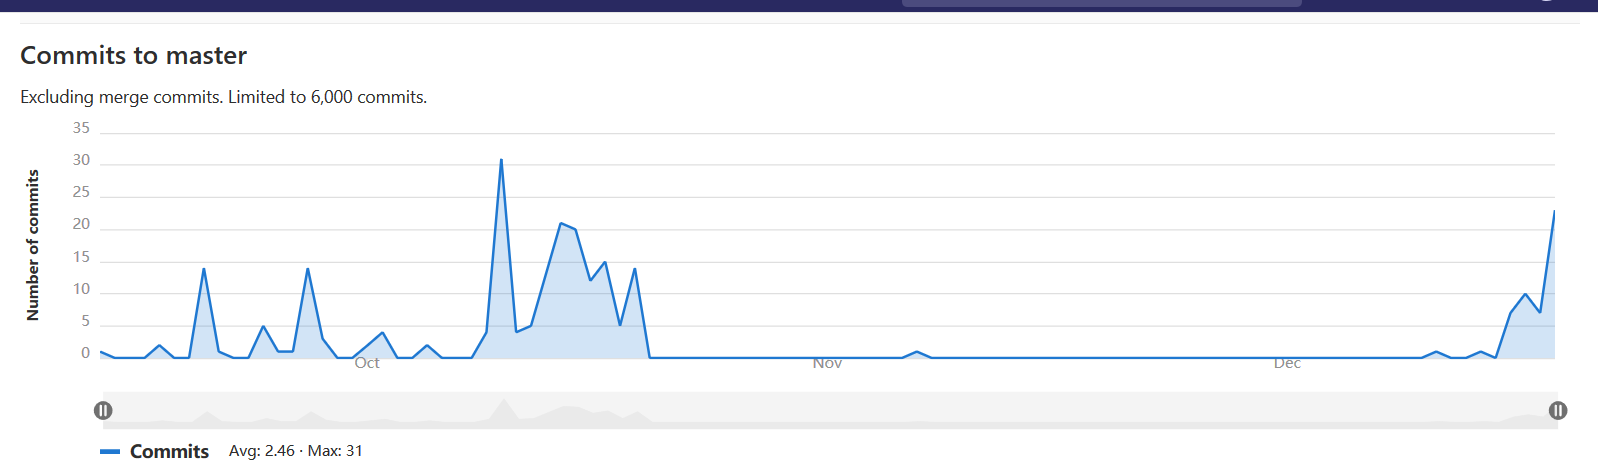
\includegraphics[width=\linewidth]{images/contribs_1.png}
			\caption{Contributors}
			\label{fig:contribs_1}
		\end{figure}
	
		\begin{figure}[H]
			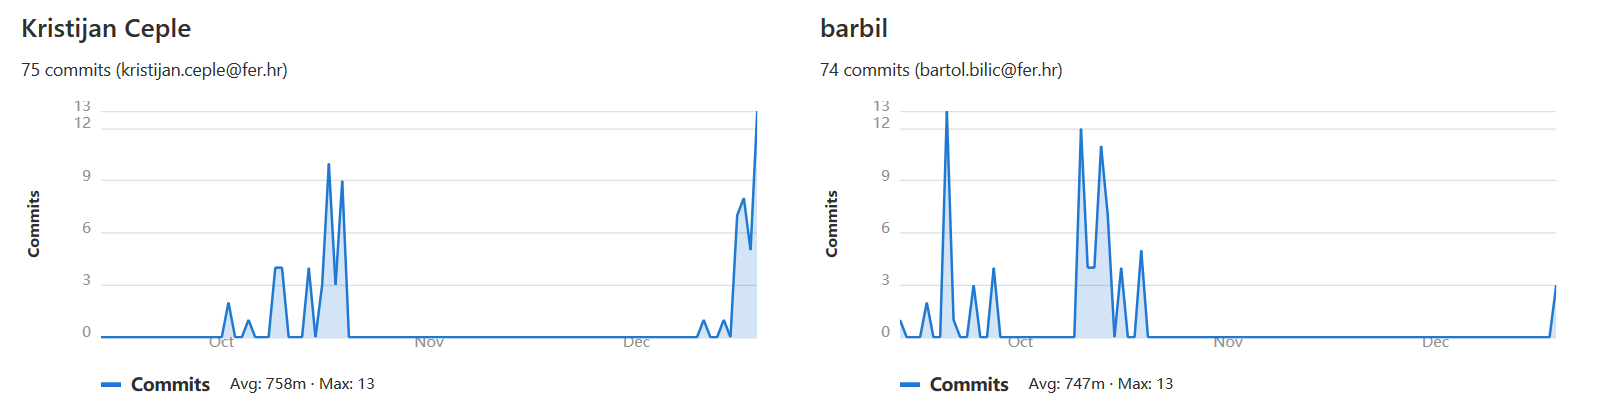
\includegraphics[width=\linewidth]{images/contribs_2.png}
			\caption{Contributors}
			\label{fig:contribs_2}
		\end{figure}

		\begin{figure}[H]
			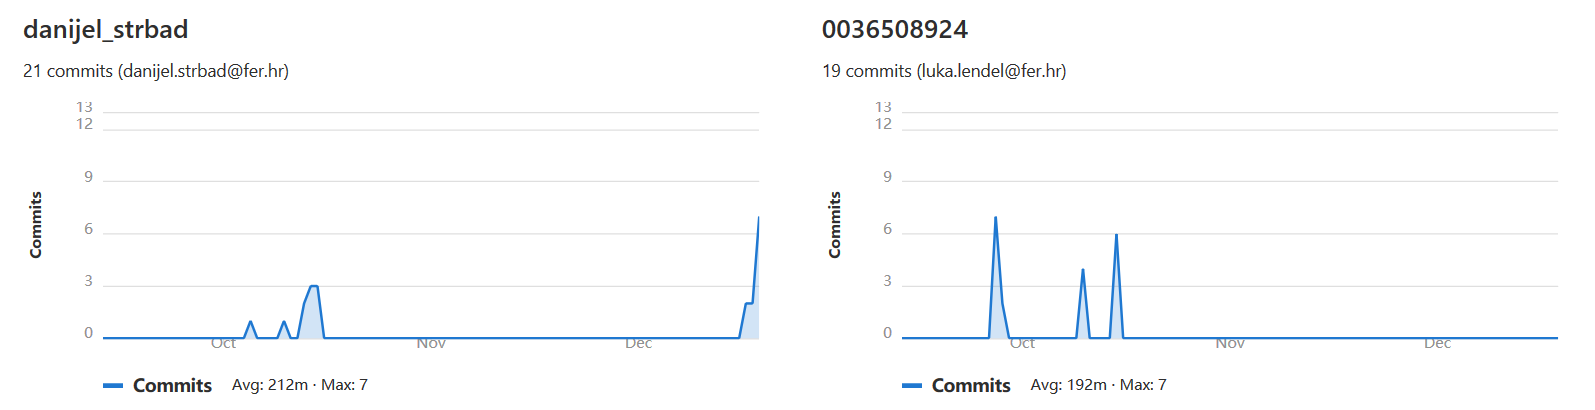
\includegraphics[width=\linewidth]{images/contribs_3.png}
			\caption{Contributors}
			\label{fig:contribs_3}
		\end{figure}

		\begin{figure}[H]
			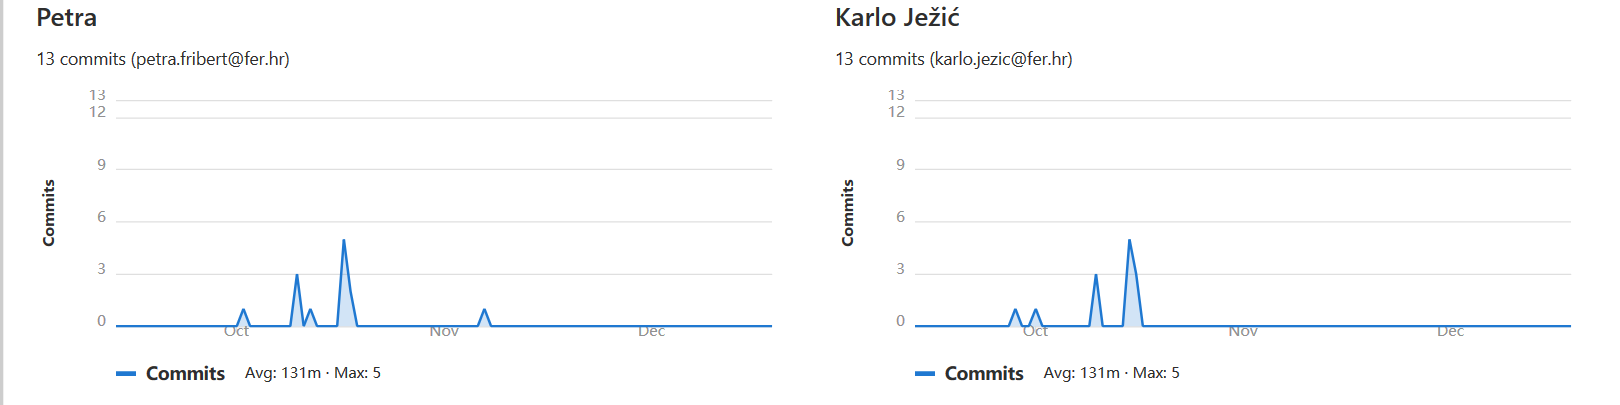
\includegraphics[width=\linewidth]{images/contribs_4.png}
			\caption{Contributors}
			\label{fig:contribs_4}
		\end{figure}

		\begin{figure}[H]
			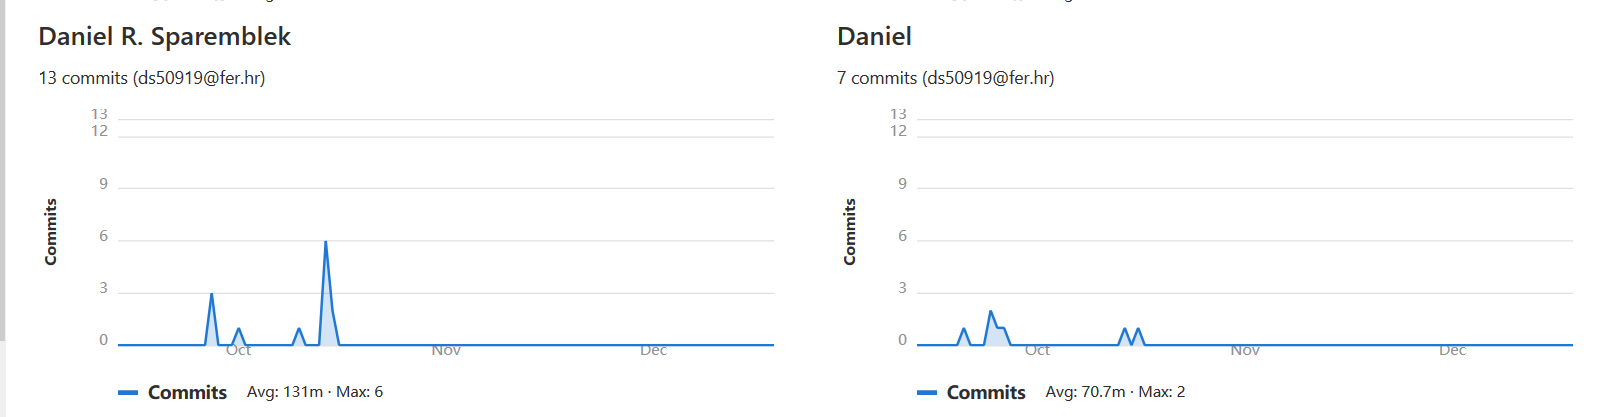
\includegraphics[width=\linewidth]{images/contribs_5.png}
			\caption{Contributors}
			\label{fig:contribs_5}
		\end{figure}

		\begin{figure}[H]
			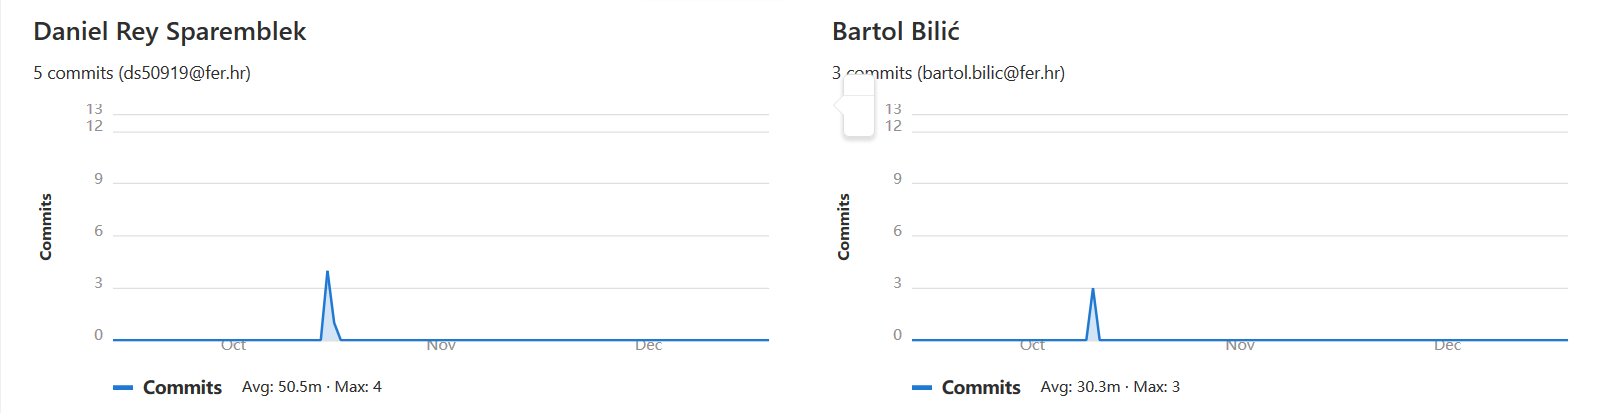
\includegraphics[width=\linewidth]{images/contribs_6.png}
			\caption{Contributors}
			\label{fig:contribs_6}
		\end{figure}

		\begin{figure}[H]
			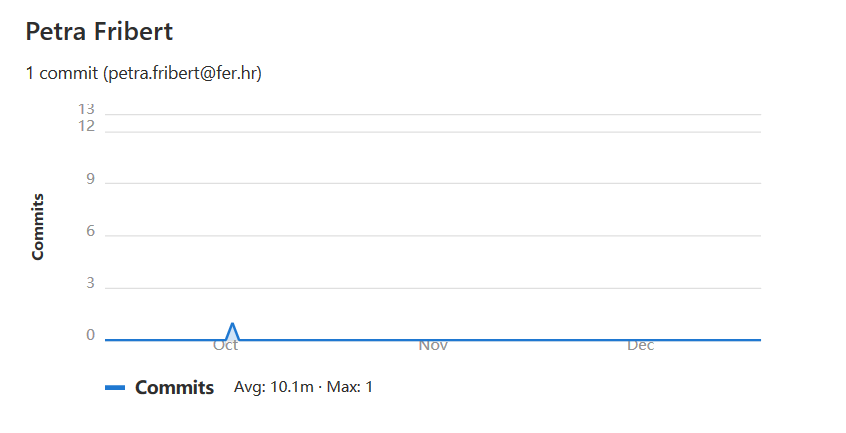
\includegraphics[width=\linewidth]{images/contribs_7.png}
			\caption{Contributors}
			\label{fig:contribs_7}
		\end{figure}
		
	